\documentclass[informe.tex]{subfiles}
\begin{document}

En general, un sistema de procesamiento de señales digitales se puede representar como se muestra en el diagrama, Fig. \ref{fig:construccion:diagr_diagr_bloques_dsp}. El bloque de conversión  a digital, ADC, muestrea y cuantifica la señal analógica $\tilde{x}(t)$  en una secuencia de tiempo discreto $x(n)$, seguido \underline{se trata la señal digital mediante algún algoritmo de procesamiento digital, DSP,} y finalmente se reconstruye la secuencia discreta resultante $y(n)$ en una señal de analógica de tiempo continuo $y(t)$. Adicionalmente se incluyen filtros limitadores de frecuencia en cada uno de los extremos, uno en la entrada con el fin de rechazar el ingreso de frecuencias indeseadas, que van a estar por encima de la mitad de la frecuencia muestreo del sistema, y otro filtro limitador en la salida para descartar las componentes de frecuencia superiores y así suavizar la salida.\newline

	\begin{figure}[h]
		\centering
		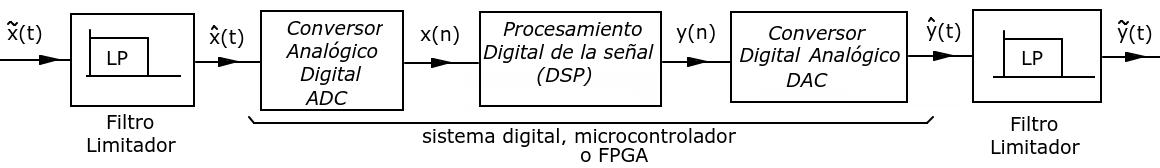
\includegraphics[scale=0.4]{construccion_diagr_bloques_dsp.jpg}
		\caption{Diagrama de bloques, procesamiento digital de señales}
		\label{fig:construccion:diagr_diagr_bloques_dsp}
	\end{figure}

El algoritmo computacional de un filtro digital puede ser construido mediante un \underline{hardware de propósito general} o \underline{un hardware de dedicado}. En un hardware dedicado, los elementos básicos computacionales, como las sumas, multiplicación por constantes y retardos se implementan mediante compuertas y unidades de memorias, ya sea con componentes discretos o integrados en un microcircuito. Otra forma de representar estos algoritmos es por medio de software, ejecutado en algún hardware de propósito general, como puede ser un microcontrolador o una computadora personal.\newline

\textbf{Construcción mediante software, ejecutado por medio de un microcontrolador}\newline

La implementación del algoritmo de un filtro digital puede haber ligeras variaciones entre una y otra, dependiendo del lenguaje de programación, la técnica de bufferización que ofrezca el hardware, etc. Por ejemplo, los microcontroladores avanzados traen instrucciones especiales de procesamientos de señales, conocidos como DSP. Estas instrucciones pueden ser como, por ejemplo, la convolución de señales.\newline

Una representación general del sistema en bloques se muestra en la Fig. \ref{fig:construccion:software}. Los bloques ADC, y DAC son hardware especifico, que en la mayoría de los casos se incluye junto al microcontrolador, en el mismo microcircuito. El bloque de procesamiento es implementado mediante rutinas de software.\newline  

	\begin{figure}[h]
		\centering
		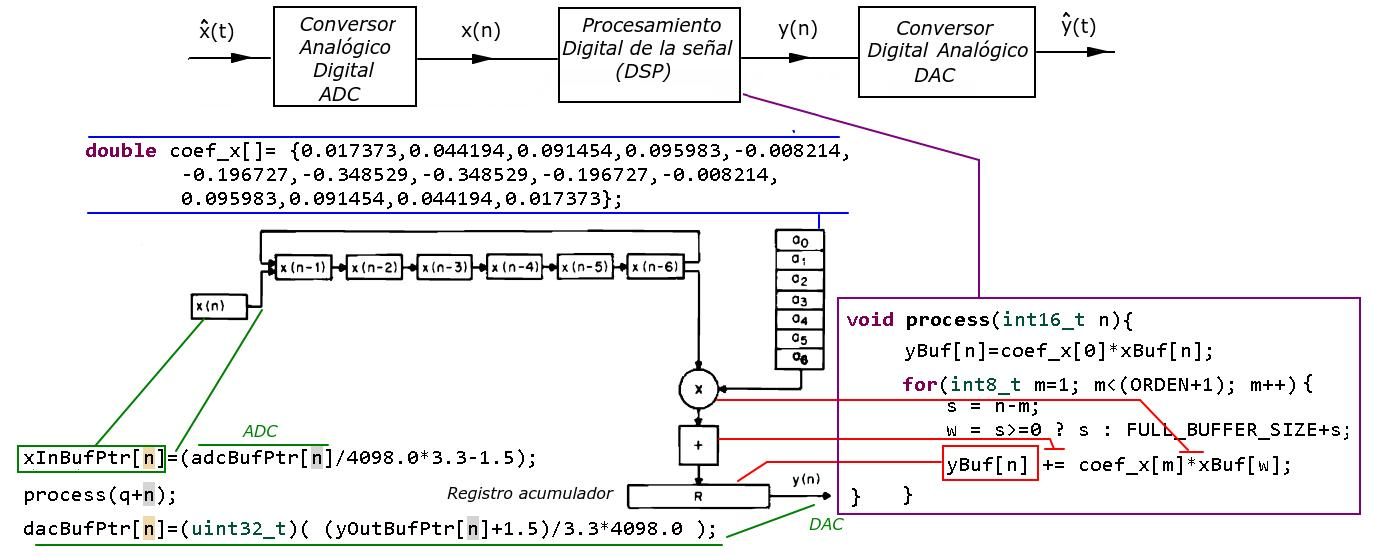
\includegraphics[scale=0.5]{construccion_software.jpg}
		\caption{Representación del algoritmo de un filtro FIR, rutinas en c correspondientes al proceso, asociado al diagrama general de procesamiento digital, \ref{fig:construccion:diagr_diagr_bloques_dsp} }
		\label{fig:construccion:software}
	\end{figure}

En la Fig. \ref{fig:construccion:software}, se muestra de forma simplificada las rutinas asociadas al bloque DSP de un filtro FIR con su lista de coeficientes, y superpuesto a este diagrama se asocia otro diagrama de bloques que representa el algoritmo completo del filtro.\\


\textbf{Construcción mediante hardware específico}\newline

En la construcción de un filtro con componentes discretos o un microcircuito que integre el diseño con componentes discretos se pueden presentar dificultades prácticas, esto es porque para el primero se necesita cablear una enorme cantidad de componentes y para el segundo, las dificultades  pueden ser simplemente por la imposibilidad de acceso a la tecnología necesaria. Una alternativa viable es la utilización de FPGAs (o tecnologías similares).\\

Las FPGAs y similares consisten en un microcircuito con una enorme cantidad de celdas lógicas configurables. Así se pueden construir mediante algún lenguaje de especificación de hardware directamente o indirectamente (por medio de un esquemático) circuitos digitales de diversas complejidades.\\

Dependiendo del entorno de desarrollo que se utilice se puede ir definiendo los bloques fundamentales del filtro y luego ir interconectándolos hasta lograr el filtro de las características deseadas.\\

En la Fig. \ref{fig:construccion:hardware:fpga:adc} se muestra cada uno del conjunto de bloques representativos junto con el código de descripción de hardware para cada una de las operaciones básicas necesarias para la implementación del hardware. Estos bloques forman parte del filtro construido que se muestra en la Fig. \ref{fig:disenio_y_construccion:fpga:board:arq}.\\

\begin{figure}[h!]
    \centering
    \begin{subfigure}[b]{1\textwidth}
         \centering
         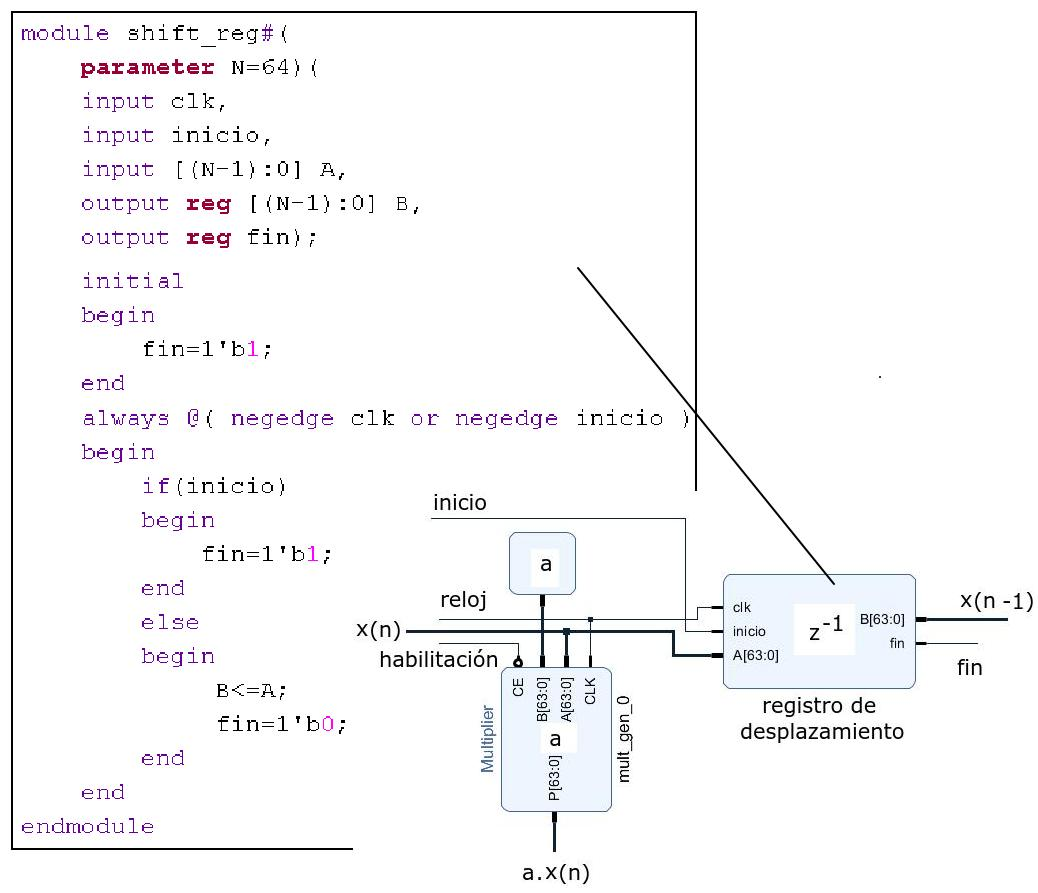
\includegraphics[scale=0.4]{construccion_hardware_retardo.jpg}
         \caption{Representación del bloque de retardo y del bloque de multiplicación de una constante por la señal}
         \label{fig:construccion:hardware:fpga:retardo}
    \end{subfigure}
\end{figure}

\begin{figure}[h]
	\ContinuedFloat
    \begin{subfigure}[b]{1\textwidth}
         \centering
         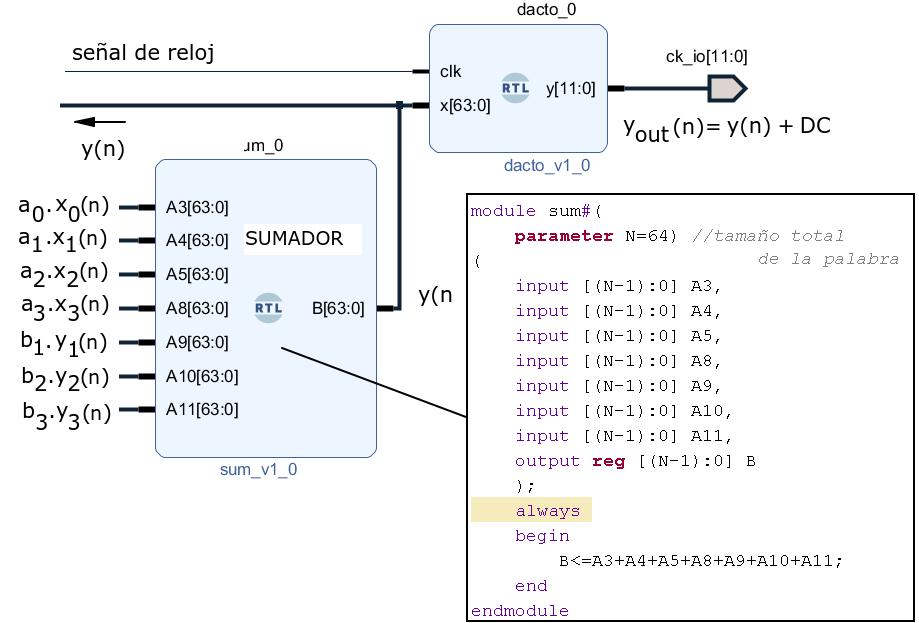
\includegraphics[scale=0.4]{construccion_hardware_suma.jpg}
         \caption{Implementación del bloque sumador de señales y representación del bloque DAC}
         \label{fig:construccion:hardware:fpga:suma_dac}
    \end{subfigure}
\end{figure}
   
\begin{figure}[h] 
	\ContinuedFloat   
    \begin{subfigure}[b]{1\textwidth}
         \centering
         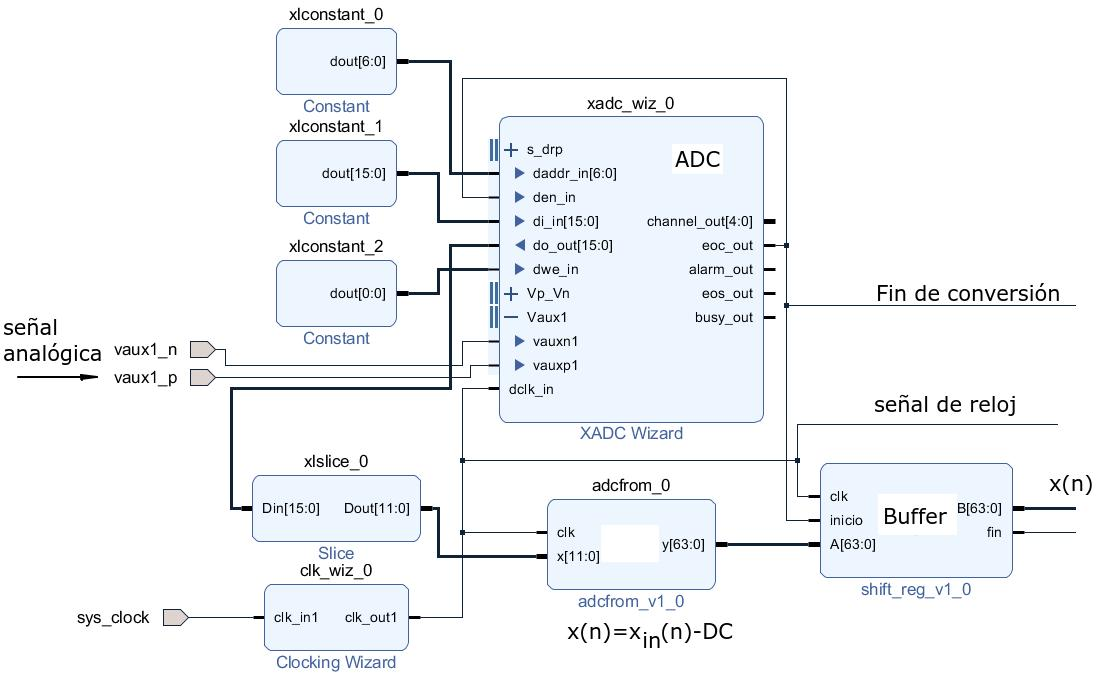
\includegraphics[scale=0.6]{construccion_hardware_adc.jpg}
         \caption{Representación del bloque ADC}
         \label{fig:construccion:hardware:fpga:adc}
    \end{subfigure}
    \caption{Implementación de los bloques de operaciones mediante FPGA}
    \label{fig:construccion:hardware:fpga:adc}    
\end{figure}


\end{document}	